\documentclass[a4paper,10pt]{scrartcl}
\usepackage[ngerman]{babel}
\usepackage{graphicx}
\usepackage{mathtools}

\usepackage{scrlayer-scrpage}
\lohead{Aufgabe 5: Rominos}
\rohead{Team-ID: ***REMOVED***}
\cfoot*{\thepage{}}

\usepackage{listings}
\usepackage{color}
\definecolor{mygreen}{rgb}{0,0.6,0}
\definecolor{mygray}{rgb}{0.5,0.5,0.5}
\definecolor{mymauve}{rgb}{0.58,0,0.82}
\lstset{
  keywordstyle=\color{blue},
  commentstyle=\color{mygreen},
  stringstyle=\color{mymauve},
  rulecolor=\color{black},
  basicstyle=\footnotesize\ttfamily,
  numberstyle=\tiny\color{mygray},
  literate=%
  {Ö}{{\"O}}1
  {Ä}{{\"A}}1
  {Ü}{{\"U}}1
  {ß}{{\ss}}1
  {ü}{{\"u}}1
  {ä}{{\"a}}1
  {ö}{{\"o}}1
  {░}{{ }}1
  {█}{{X}}1
}

\title{Aufgabe 5: Rominos}
\author{Team-ID: ***REMOVED*** \\\\
	    Team-Name: ***REMOVED*** \\\\
	    Bearbeiter dieser Aufgabe: \\
	    ***REMOVED***\\\\}
\date{\today}

\begin{document}

\maketitle
\tableofcontents

\section{Lösungsidee}
Zur lösung der Aufgabe generiere ich alle gültigen Rominos der Größe n und sortiere dann die deckungsgleichen Rominos aus.

\section{Umsetzung}
Ich stelle mir alle Rominos in einem Koordinatensystem mit dem Ursprung oben links vor.

Um alle gültigen Rominos einer Größe zu generieren, gehe ich von Quadrat zu Quadrat. Ich beginne mit dem Quadrat am Ursprung des Koordinatensystem und nehme dann alle positiven und diagonalen Nachbarn als Nachfolgequadrate. Ich nehme als erstes nur diagonale Nachbarn, damit die Anforderung von mindestens einer diagonalen Verbindung bereits abgedeckt ist. Bei weiteren Quadraten nehme ich auch gerade Nachbarn.

\begin{figure}[h]
  \centering
  
\includegraphics{raute.jpg}
  \caption{Der 4er-Rautenromino}
  \label{fig:raute}
\end{figure}

Alle Rominos außer die "Raute" (siehe Abbildung \ref{fig:raute}) können von dem Quadrat mit der Position \((0|0)\) aus generiert werden. Damit auch die "Raute" generiert werden kann verwende ich als Startquadrat auch die Positionen bis \((0|\frac{n}{2}-1)\). Bei \(n=4\) währen das die Positionen \((0|0)\) und \((0|1)\).

Mit dem letzten Quadrat, das für einen Romino generiert wird muss der Romino, mindestens ein Quadrat mit \(x=0\) und mindestens ein Quadrat mit \(y=0\) haben, damit das spätere Verschieben der Rominos nicht nötig ist.

Um die deckungsgleichen Rominos aus zu sortieren, generiere ich der Reihe nach für jeden Romino die gespiegelt, gedrehte und gespiegelt-drehte Version des Rominos, wenn der Romino mit keiner gespiegelt, gedrehten oder gespiegel-drehten Version eines anderen Romino übereinstimmt ist er nicht deckungsgleich und ein weitere Romino der Größe n.

Am Ende des Programms werden alle gefunden Rominos optinal in eine Ausgabedatei gespeichert.
\pagebreak

\section{Beispiele}
Hier werde ich die Beispiele aus der Aufgabe aufführen (\(n=4,...,10\)) und am Ende noch zwei eigene Beispiele.

\subsection{Beispiel \(n=4\)}
17 Rominos der Größe \(n=4\) \\\\
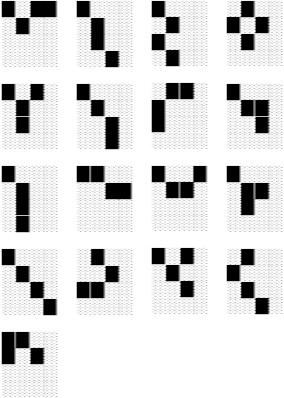
\includegraphics{4.jpg}
\pagebreak

\subsection{Beispiel \(n=5\)}
82 Rominos der Größe \(n=5\) \\\\
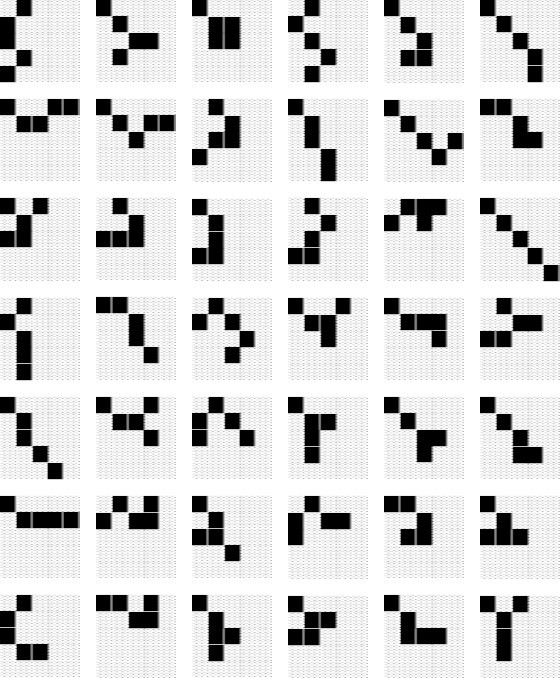
\includegraphics{5a.jpg} \\
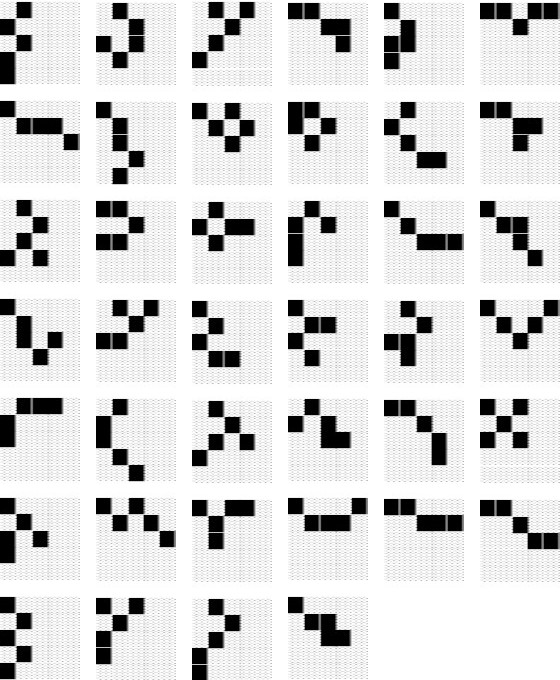
\includegraphics{5b.jpg}

\subsection{Beispiel \(n=6\)}
485 Rominos der Größe \(n=6\)

\subsection{Beispiel \(n=7\)}
2892 Rominos der Größe \(n=7\)

\subsection{Beispiel \(n=8\)}
18116 Rominos der Größe \(n=8\)

\subsection{Beispiel \(n=9\) und \(n=10\)}
Mir war es nicht möglich mit meinem Programm und meinem PC die 9er- und 10er-Rominos zu berechnen, weil ich nicht genug Arbeitsspeicher zu verfügung habe.

Bei n=9 müssten es sich um die 100 Tausend Rominos handeln und bei n=10 um die Millionen. Diese Annahme ziehe ich aus dem Verhältnis 1 zu 10 der Ergebnisse für die 7er und 8er-Rominos.

\subsection{Beispiel \(n=2\)}
Bei \(n=2\) gibt es nur einen Romino, der auch mit meinem Programm gefunden werden kann: \\\\

\includegraphics{2.jpg}

\subsection{Beispiel \(n=1\)}
Bei \(n=1\) gibt es keinen Romino, weil mit nur einem Quadrat keine diagonale Verbindung möglich ist.

\section{Quellcode}
\lstset{numbers=left}
\lstinputlisting[language=python]{Aufgabe5:Rominos/rominos.py}

\end{document}
